\subsection{UC15 - Telegram - Notifiche Push}
		
		%\begin{figure}[t!]
		%	\centering
		%	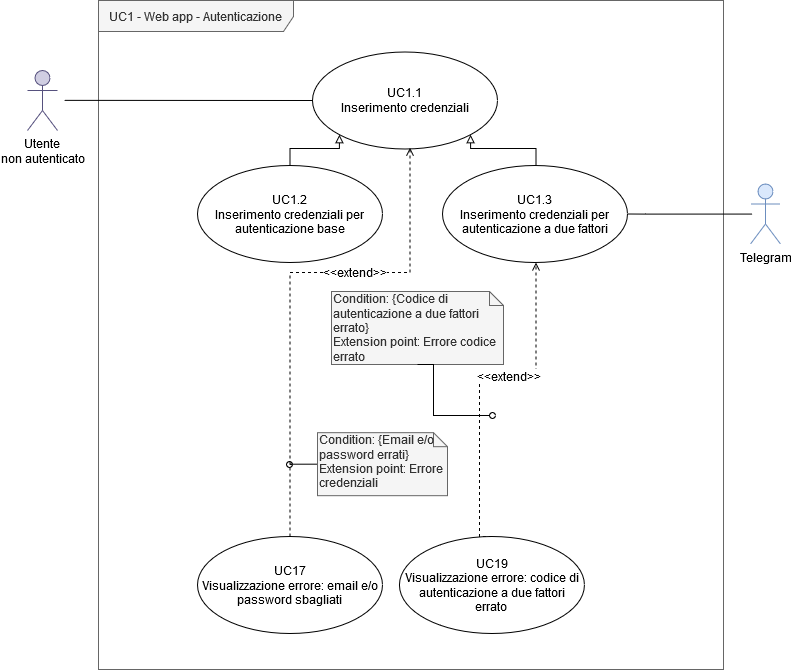
\includegraphics[height=10em]{res/images/uc1}
		%\end{figure}
		
	\begin{itemize}
		\item \textbf{Attori Primari}: Membro, Moderatore ente, Amministratore.
		\item \textbf{Attori Secondari}: \glock{Telegram}.
		\item \textbf{Descrizione}: Un utente, con l'applicazione di \glock{Telegram} attiva o in background, riceve una notifica push in base a un evento nel sistema. 
		\item \textbf{Precondizione}: L'utente ha l'applicazione di \glock{Telegram} attiva o in background e ha una chat autenticata con il bot.
		\item \textbf{Postcondizione}: L'utente riceve una notifica da parte di \glock{Telegram}.
		\item \textbf{Scenario Principale}:
		\begin{enumerate}
			\item L'utente ha l'applicazione di \glock{Telegram} attiva o in background. 
			\item L'utente riceve una notifica push come messaggio di testo nella chat autorizzata con il Bot.
		\end{enumerate}
	\end{itemize}
	
	\subsubsection{UC 15.1 - Ricezione notifica alert}

	\begin{itemize}
		\item \textbf{Attori Primari}: Membro, Moderatore ente, Amministratore.
		\item \textbf{Attori Secondari}: \glock{Telegram}.
		\item \textbf{Descrizione}: L'utente riceve una notifica sulla chat con il bot di \glock{Telegram} relativa ad un alert in cui un sensore ha superato una soglia prevista.
		\item \textbf{Precondizione}: L'utente ha l'applicazione di \glock{Telegram} attiva o in background e ha una chat autenticata con il bot.
		\item \textbf{Postcondizione}: L'utente riceve una notifica come messaggio di testo in chat con le informazioni relative all'alert.
		\item \textbf{Scenario Principale}:
		\begin{enumerate}
			\item L'utente ha l'applicazione di \glock{Telegram} attiva o in background.
			\item L'utente riceve una notifica che riguarda un alert nella chat con il bot.
		\end{enumerate}
	\end{itemize}

	\subsubsection{UC 15.2 - Ricezione codice di autenticazione a due fattori}

	\begin{itemize}
		\item \textbf{Attori Primari}: Membro, Moderatore ente, Amministratore.
		\item \textbf{Attori Secondari}: \glock{Telegram}.
		\item \textbf{Descrizione}: L'utente riceve una notifica sulla chat con il bot di \glock{Telegram} relativa al codice di autenticazione a due fattori mentre sta svolgendo l'autenticazione nella web app.
		\item \textbf{Precondizione}: L'utente ha l'applicazione di \glock{Telegram} attiva o in background e ha una chat autenticata con il bot.
		\item \textbf{Postcondizione}: L'utente riceve una notifica come messaggio di testo in chat con le informazioni relative al codice a due fattori.
		\item \textbf{Scenario Principale}:
		\begin{enumerate}
			\item L'utente ha l'applicazione di \glock{Telegram} attiva o in background.
			\item L'utente riceve una notifica che riguarda il codice di autenticazione a due fattori da usare come credenziale per accedere alla web app.
		\end{enumerate}
	\end{itemize}